\documentclass[12pt]{report}
\usepackage[french]{babel}
\usepackage[utf8]{inputenc}
\usepackage{amsmath, amsthm, amssymb, amsfonts}
\usepackage{graphicx}
\usepackage[colorinlistoftodos]{todonotes}
\usepackage{color}
\usepackage{pifont}
\usepackage[Glenn]{fncychap} %Conny, Glenn, Bjarne, Bjornstrup, Rejne, Lenny
\frenchbsetup{StandardLists=true}
%\usepackage[a4paper,pdftex]{geometry}	% Use A4 paper margins
\usepackage[french]{babel}
\usepackage{multicol}
\usepackage[version=3]{mhchem}
\usepackage{hyperref} 
\usepackage[a4paper,pdftex,left=2.5cm,right=2.5cm,top=2.5cm,bottom=2.5cm]{geometry}
\usepackage[section]{placeins} 
\usepackage{float} 
\usepackage{here}
 
 
\definecolor{orange}{cmyk}{0,0.5,1,0}
\definecolor{forestgreen}{rgb}{0.13,0.54,0.13}
\definecolor{carmine}{rgb}{0.59, 0.0, 0.09}
\definecolor{grey}{rgb}{0.5,0.5,0.5}
\definecolor{blue}{rgb}{0.2, 0.2, 0.6}


\begin{document}

\renewcommand{\arraystretch}{1.5}

{\textcolor{carmine}{\chapter{Introduction}}}

Dans le cadre de la deuxième thématique abordée durant notre projet, à savoir la gestion de la production, il nous a été demandé de faire varier certains paramètres du procédé afin d'analyser leurs effets sur : \\
\begin{itemize}
\item La production de $NH_3$, ceci étant notre but premier.
\item Les débits intermédiaires.
\item Le débit de $CO_2$, son caractère polluant étant loin d'être négligeable. Cependant nous avons appris lors de notre visite à Yara\footnote{Dans le cadre du projet, différentes visites ont été proposées. L'une d'elles était la visite du centre de production d'amoniac Yara à Tertre.} qu'il était possible de revendre celui-ci afin de rendre sa production utile. Par exemple dans l'industrie alimentaire. 
\item Le volume d'air à traiter, la séparation de celui-ci étant énergivore et coûteuse.
\end{itemize}

Nous allons faire varier les paramètres suivants dans les plages de valeurs indiquées : \\


\begin{tabular}{|l|c|}
\hline
Rapport molaire $\frac{O_2}{CH_4}$ à l'entrée de l'ATR & 0.2 - 0.8 \\
\hline
Rapport molaire $\frac{H_2O}{CH_4}$ à l'entrée de l'ATR & 0.5 - 4 \\
\hline
Température de sortie de la zone de reforming de l'ATR & 1000 - 1600 [K]\\
\hline
Pression d'opération de l'ATR & 20 - 100 [bar] \\
\hline
\end{tabular}
\bigskip

Pour réaliser notre analyse, nous avons choisi de nous concentrer chaque fois sur une conséquence possible de la variation des paramètres afin de faire clairement ressortir nos possibilités d'action sur ceux-ci.\\
Pour chaque variation, nous avons ressorti les graphes correspondants de notre outil de calcul matlab.\\




{\textcolor{carmine}{\chapter{Influence sur le débit final de $NH_3$}}}



\section{Variation du ratio molaire $\frac{O_2}{CH_4}$}

Grâce au graphe de la figure 1.1 ci dessous, nous avons pu constater que le débit de $NH_3$ est maximum lorsque le ratio molaire $\frac{O_2}{CH_4}$ est à sa plus petite valeur, c'est à dire $0,2$. Cette valeur implique que la concentration molaire en $CH_4$ soit 5 fois plus élevée que celle en $O_2$.

\begin{figure}[H]
\begin{center}
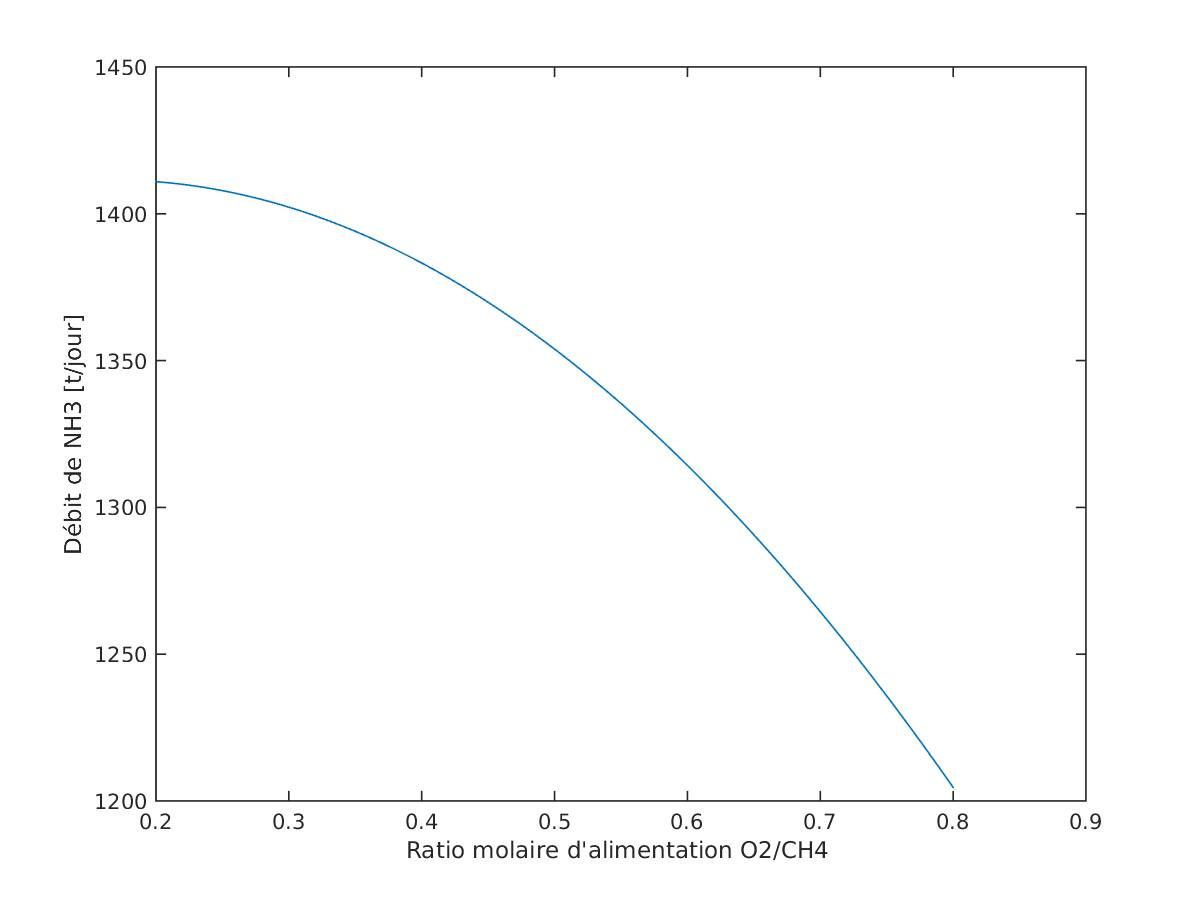
\includegraphics[scale=0.3]{debit_NH3_ratio_O2}
\caption{Evolution du débit de sortie de $NH_3$ en fonction du ratio molaire $\frac{O_2}{CH_4}$}
\end{center}
\end{figure}

Ce phénomène s'explique par le fait que l'$O_2$ n'intervient que dans la toute première réaction dans l'ATR, la combustion, que nous considérons comme complète :

\begin{equation}
 CH_4 + 2O_2 \rightarrow CO_2 + 2H_2O
\end{equation}

 
 Alors que le $CH_4$, quant à lui intervient également dans les deux réactions simultanées :
 
 \begin{equation}
 CH_4 + H_2O \leftrightarrow 3H_2 + CO
 \end{equation}
 \begin{equation}
 CO + 2H_2O \leftrightarrow H_2 + CO_2
 \end{equation}

La réaction (2.1) étant considérée complète, le nombre de moles réagissant est déterminé par le réactif limitant. Dans les plages de valeurs que nous utilisons, ce réactif sera toujours l'$O_2$. Au moins le nombre de moles d'$O_2$ est élevé, au plus il restera du $CH_4$ prêt à réagir avec l'$H_2O$ pour former du $CO_2$ et du $H_2$.\\

Or, le $H_2$ est indispensable à l'étape finale, la synthèse de l'amoniac : 
\begin{equation}
N_2 + 3H_2 \rightarrow 2NH_3
\end{equation}
L'azote, $N_2$, étant obtenu par séparation de l'air et étant 4 fois plus présent dans ce dernier que l'oxygène, est présent en suffisance pour les quantités de $H_2$ prêtes à réagir\footnote{Dans notre outil, selon nos hypothèses}. Dès lors, au plus il y a de $H_2$, au plus nous obtenons du $NH_3$, notre objectif final.\\

Cela explique donc la forme du graphe obtenu.\\

\section{Variation du ratio molaire $\frac{H_2O}{CH_4}$}

Sur le graphe de la figure 2.2 ci-dessous, il apparaît clairement que le débit de $NH_3$ augmente avec le ratio molaire d'alimentation $\frac{H_2O}{CH_4}$.\\

\begin{figure}[H]
\begin{center}
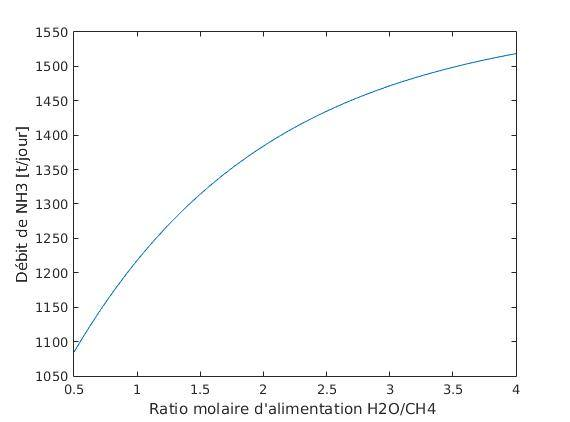
\includegraphics[scale=0.6]{debit_NH3_ratio_H2O}
\caption{Evolution du débit de sortie de $NH_3$ en fonction du ratio molaire $\frac{H_2O}{CH_4}$}
\end{center}
\end{figure}

Cela s'explique principalement par la réaction de formation du $H_2$ qui a lieu dans le WGS : 
\begin{equation}
CO + H_2O \rightarrow H_2 + CO_2
\end{equation}
Etant donné que nous considérons cette réaction comme complète,  c'est le réactif limitant qui détermine le nombre de moles de $H_2$ obtenues et, via l'intervention du $H_2$ dans l'étape finale, la quantité de $NH_3$.\\

Le CO produit dépendant en partie de la quantité d'$H_2O$ entrant dans l'ATR, il est proportionnel au flux entrant de ce dernier. Il est donc normal d'observer une augmentation du débit de sortie de $NH_3$ lorsqu'on augmente l'alimentation en $H_2O$, étant donné que la quantité de $H_2$ présente pour la synthèse en dépend directement.\\

\section{Variation de la pression dans l'ATR}

Les lois de la physique veulent que, lorsqu'un système est perturbé, il agira toujours dans le but de minimiser la perturbation. Si la perturbation en question est une augmentation de pression, le système va donc chercher à diminuer le nombre de moles de gaz en orientant vers le côté où il y a  le moins de moles de gaz.\\

\begin{figure}[H]
\begin{center}
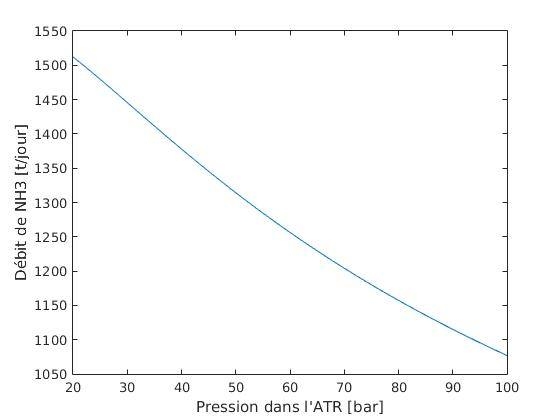
\includegraphics[scale=0.6]{debit_NH3_pression_ATR}
\caption{Evolution du débit de sortie de $NH_3$ en fonction de la pression dans l'ATR}
\end{center}
\end{figure}

La pression n'influencera pas la première réaction de l'ATR, le nombre de moles de gaz étant le même de chaque côté.\\

En ce qui concerne les deux réactions en équilibre ci-dessous, celles-ci seront dirigées dans le sens de la flèche rouge :\\

 \begin{equation}
 CH_4 + H_2O \hspace{0.5cm}\textcolor{red}{\overleftarrow{\textcolor{black}{\Longleftrightarrow}}} \hspace{0.5cm} 3H_2 + CO
 \end{equation}
 \begin{equation}
 CO + 2H_2O \hspace{0.5cm}\textcolor{red}{\overrightarrow{\textcolor{black}{\Longleftrightarrow}}} \hspace{0.5cm} H_2 + CO_2
 \end{equation}
 
 Le système d'équilibre ainsi redirigé explique le graphe obtenu d'une part car la réaction 2.6, de plus en plus dirigée vers les réactifs, produira de moins en moins de $H_2$. Or cette réaction produit la majorité du $H_2$ qui sera utilisée pour la synthèse.\\
 
 D'autre part, la réaction 2.6 produira de moins en moins de $CO$ à mesure que la pression d'opération de l'ATR augmentera. La réaction 2.7 est dirigée vers les produits mais sera limitée par la quantité en CO si celle-ci est trop faible et donc réduira le $H_2$ produit par cette deuxième réaction.\\

La diminution de la production de $NH_3$ est donc expliquée par cette diminution de production de $H_2$, diminution que nous pouvons observer sur le graphe ci-dessous :
\begin{figure}[H]
\begin{center}
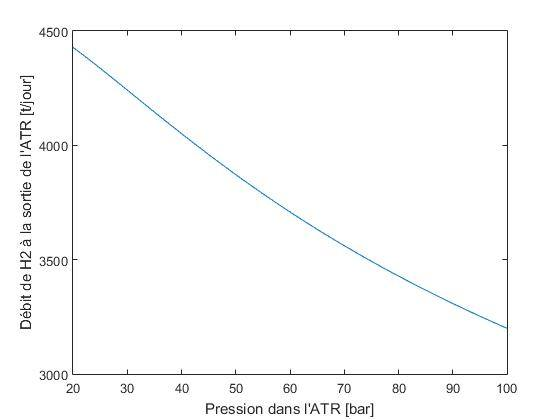
\includegraphics[scale=0.6]{debit_H2_ATR_pression_ATR}
\caption{Evolution du débit de H2 à la sortie de l'ATR en fonction de la pression dans celui-ci}
\end{center}
\end{figure}


\section{Variation de la température de la zone de reforming de l'ATR}

\textcolor{red}{\textbf{!!! INSISTER !!! + graphes avec les courbes de niveau\\
Tsortie < Tmax ATR si trop grande Tsortie, ATR appréciera pas Tmax.}}
L'énoncé de Van't Hoff 

 \begin{equation}
 CH_4 + H_2O \hspace{0.5cm}\textcolor{red}{\overrightarrow{\textcolor{black}{\Longleftrightarrow}}} \hspace{0.5cm} 3H_2 + CO \hspace{1cm}\textcolor{red}{ENDO}
 \end{equation}
 \begin{equation}
 CO + 2H_2O \hspace{0.5cm}\textcolor{red}{\overleftarrow{\textcolor{black}{\Longleftrightarrow}}} \hspace{0.5cm} H_2 + CO_2 \hspace{1cm}\textcolor{red}{EXO}
 \end{equation}


\begin{figure}[H]
\begin{center}
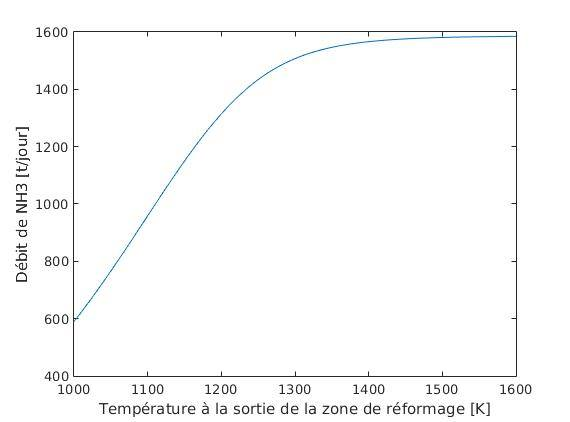
\includegraphics[scale=0.6]{debit_NH3_Temperature}
\caption{Evolution du débit de sortie de $NH_3$ en fonction de la température de la zone de reforming de l'ATR}
\end{center}
\end{figure}



\textcolor{carmine}{\chapter{Influence sur le débit de $CO_2$}}

\section{Variation du ratio molaire $\frac{O_2}{CH_4}$}

Le graphe de la figure 3.1 montre très clairement que le débit de $CO_2$ augmente quasiment linéairement avec l'augmentation du ratio molaire $\frac{O_2}{CH_4}$

\begin{figure}[H]
\begin{center}
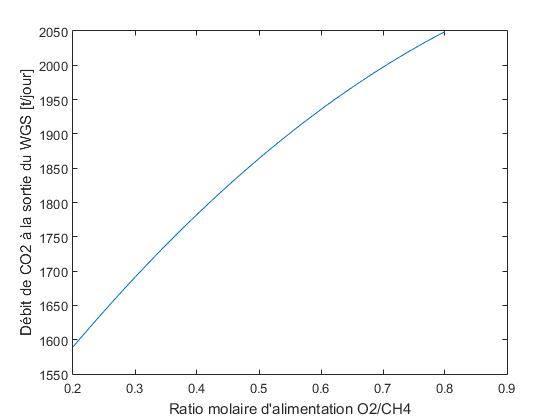
\includegraphics[scale=0.6]{debit_CO2_ratio_O2}
\caption{Evolution du débit de sortie de $CO_2$ en fonction du ratio molaire $\frac{O_2}{CH_4}$}
\end{center}
\end{figure}

Cela s'explique principalement par la réaction de combustion qui est la première à avoir lieu dans l'ATR :

\begin{equation}
 CH_4 + 2O_2 \rightarrow CO_2 + 2H_2O
\end{equation}

Au plus il y a de $O_2$ présent à l'entrée de l'ATR, au plus le nombre de moles qui réagiront au cours de la combustion sera grand et au plus la quantité de $CO_2$ produite sera élevée.\\
Le débit de sortie de $CO_2$ est majoritairement constitué de celui rejeté par cette première réaction. En effet, les deux réactions suivantes dans l'ATR se font à l'équilibre, et donc la quantité de $CO_2$ produite est moindre, même si bien présente.\\ 


\section{Variation du ratio molaire $\frac{H_2O}{CH_4}$}

Lorsque l'on augmente progressivement le ratio molaire $\frac{H_2O}{CH_4}$ on observe également une augmentation du débit de $CO_2$ à la sortie du WGS.\\

\begin{figure}[H]
\begin{center}
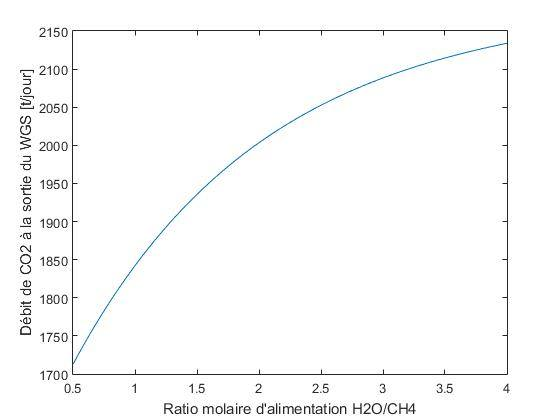
\includegraphics[scale=0.6]{debit_CO2_ratio_H2O}
\caption{Evolution du débit de sortie de $CO_2$ en fonction du ratio molaire $\frac{H_2O}{CH_4}$}
\end{center}
\end{figure}

Ce résultat est conforme à ce que nous attendions et s'explique tout d'abord par une analyse des deux réactions en équilibre dans l'ATR.
 \begin{equation}
 CH_4 + H_2O \leftrightarrow 3H_2 + CO
 \end{equation}
 \begin{equation}
 CO + 2H_2O \leftrightarrow H_2 + CO_2
 \end{equation}
 
Ces réaction produisent déjà une partie du $CO_2$ qui constituera le débit final de celui-ci. Il apparaît clairement que la quantité de $H_2O$ influe d'une part sur la production de CO, qui réagira ensuite avec le $H_2O$ qui, d'autre part, réagit pour former du $CO_2$. Le tout dans une forme d'équilibre.\\

De plus, les $H_2O$ et CO restant réagiront ensuite dans le WGS :
\begin{equation}
CO + H_2O \rightarrow H_2 + CO_2
\end{equation}
Cette réaction est complète de telle façon que tout le $CO$ réagit. Le nombre de moles de $CO_2$ formées durant cette réaction dépendant donc du nombre de moles de CO présentes, ces dernières dépendant de la quantité de $H_2O$ entrant dans le WGS.\\

Cependant, il est intéressant de remarquer la forme non linéaire du graphe. En effet, il apparaît une esquisse de limite dans l'augmentation du débit de $CO_2$ produit en fonction de la quantité de $H_2O$. Cela s'explique par le fait que la quantité de $CH_4$ présent pour réagir avec l'$H_2O$, si elle est inférieure au nombre de moles de $H_2O$ présentes, déterminera le nombre de moles qui réagiront. Donc, la limite apparait lorsque la quantité d'$H_2O$ disponible pour la réaction a dépassé la quantité de $CH_4$.\\




\section{Variation de la pression dans l'ATR}

Lorsque l'on augmente la pression d'opération de l'ATR, le débit de $CO_2$ est influencé de deux façons différentes à deux endroits du systèmes réactionnel.\\

Tout d'abord, voici le graphe du débit de $CO_2$ à la sortie de l'ATR en fonction de l'augmentation de la pression d'opération de ce dernier.

\begin{figure}[H]
\begin{center}
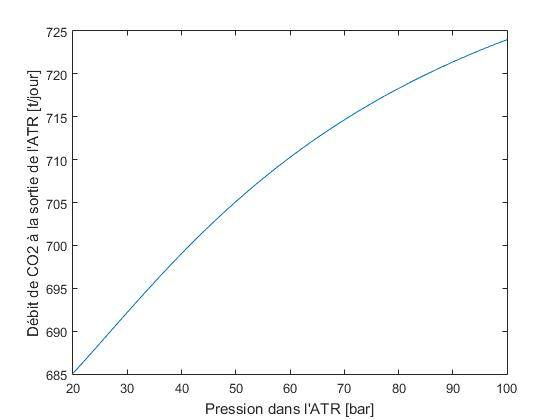
\includegraphics[scale=0.6]{debit_CO2_ATR_pression_ATR}
\caption{Evolution du débit de sortie de l'ATR de $CO_2$ en fonction de la pression dans l'ATR}
\end{center}
\end{figure}

Ce graphe montre une nette augmentation du débit de $CO_2$ à la sortie de l'ATR qui s'explique au moyen des mêmes principes de physique que ceux  évoqués au point 2.3, les équilibres des deux dernières équations de l'ATR seront influencés de la manière suivante :\\

 \begin{equation}
 CH_4 + H_2O \hspace{0.5cm}\textcolor{red}{\overleftarrow{\textcolor{black}{\Longleftrightarrow}}} \hspace{0.5cm} 3H_2 + CO
 \end{equation}
 \begin{equation}
 CO + 2H_2O \hspace{0.5cm}\textcolor{red}{\overrightarrow{\textcolor{black}{\Longleftrightarrow}}} \hspace{0.5cm} H_2 + CO_2
 \end{equation}

L'augmentation de la production de $CO_2$ dans l'ATR est donc expliquée par la réaction 2.13, qui favorise de plus en plus les produits à mesure que la pression augmente. La production de $CO_2$ est donc favorisée car la réaction se rapprochera de plus en plus d'une réaction complète.\\

D'autre part, le graphe ci-dessous nous montre que le débit final de $CO_2$ diminue très nettement avec l'augmentation de pression. Ceci est dû à la réaction qui se produit dans le WGS.
\begin{equation}
CO + H_2O \rightarrow H_2 + CO_2
\end{equation}
Cette réaction considérée comme complète produit une grande partie du $CO_2$ total rejeté. Elle dépend de l'$H_2O$ et du CO qui sortent du WGS et qui sont donc prêts à réagir.\\
Or, la réaction 2.12 favorise largement les produits et donc diminue de plus en plus la production en CO à mesure que la pression augmente. La réaction 2.13 favorise la réaction du CO, alors que la quantité disponible est déjà amoindrie.\\
Cela implique une quantité de moins en moins grande de CO dans le WGS et donc de moins en moins de $CO_2$ produit par celui-ci.\\
La quantité de $CO_2$ produite par l'ATR étant bien à bien moindre échelle que celle produite par le WGS, cela explique le graphe obtenu.\\

\begin{figure}[H]
\begin{center}
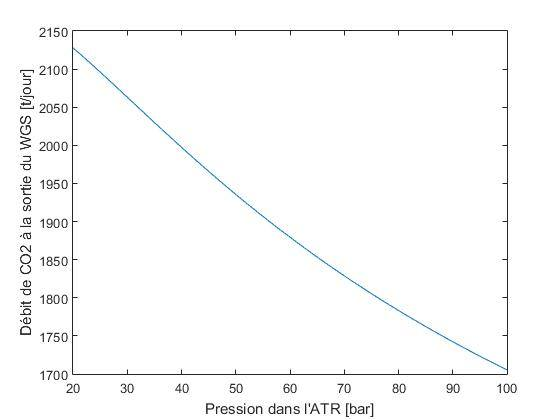
\includegraphics[scale=0.6]{debit_CO2_pression_ATR}
\caption{Evolution du débit de sortie de $CO_2$ en fonction de la pression dans l'ATR}
\end{center}
\end{figure}
 






\section{Variation de la température de la zone de reforming de l'ATR}

\begin{figure}[H]
\begin{center}
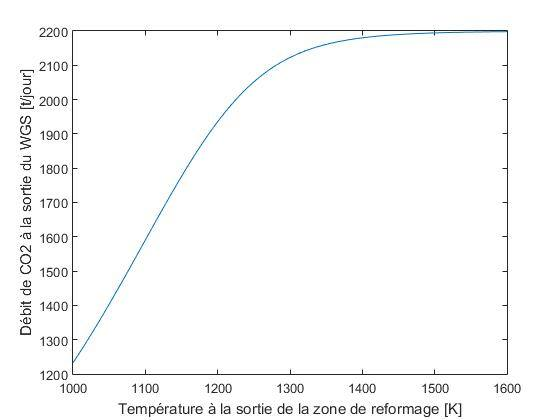
\includegraphics[scale=0.6]{debit_CO2_Temperature}
\caption{Evolution du débit de sortie de $CO_2$ en fonction de la température de sortie de la zone de reforming de l'ATR}
\end{center}
\end{figure}


\textcolor{carmine}{\chapter{Influence sur la température maximale de l'ATR}}

\section{Variation du ratio molaire $\frac{O_2}{CH_4}$}



\begin{figure}[H]
\begin{center}
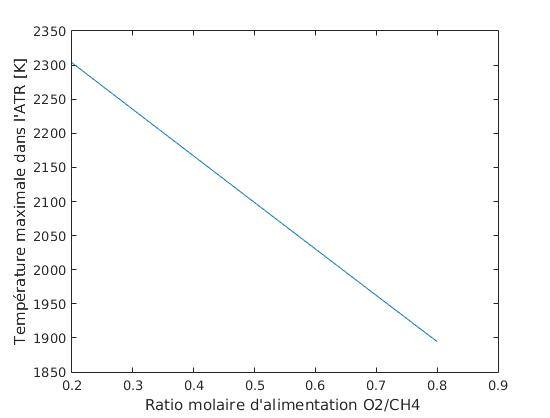
\includegraphics[scale=0.6]{Tmax_ratio_O2}
\caption{Evolution de la température maximale de l'ATR en fonction du ratio molaire $\frac{O_2}{CH_4}$}
\end{center}
\end{figure}


\section{Variation du ratio molaire $\frac{H_2O}{CH_4}$}


\begin{figure}[H]
\begin{center}
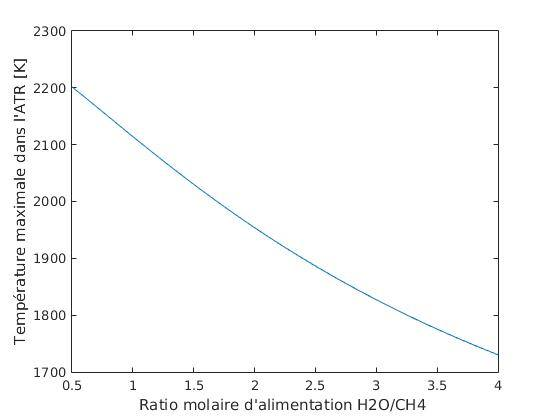
\includegraphics[scale=0.6]{Tmax_ratio_H2O}
\caption{Evolution de la température maximale de l'ATR en fonction du ratio molaire $\frac{H_2O}{CH_4}$}
\end{center}
\end{figure}

\section{Variation de la pression dans l'ATR}

\begin{figure}[H]
\begin{center}
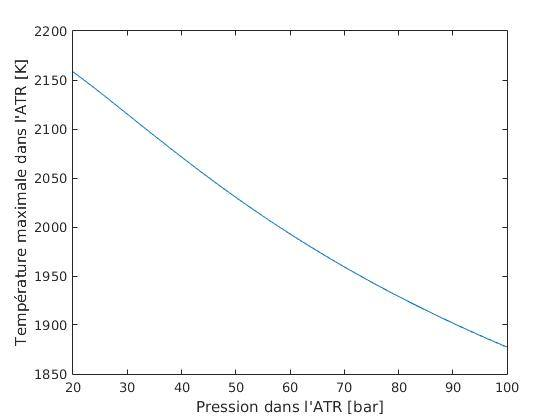
\includegraphics[scale=0.6]{Tmax_pression_ATR}
\caption{Evolution de la température maximale de l'ATR en fonction de la pression dans l'ATR}
\end{center}
\end{figure}

\section{Variation de la température de la zone de reforming de l'ATR}

Pour thématique 4 dans laquelle il nous a été demandé de planifier l'arrêt du réacteur, il nous a été demandé 

\begin{figure}[H]
\begin{center}
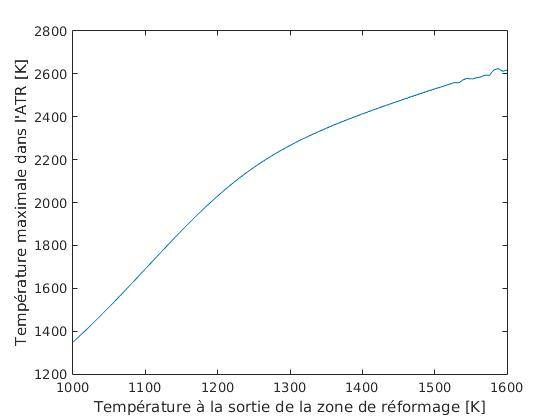
\includegraphics[scale=0.6]{Tmax_Tsortie}
\caption{Evolution de la température maximale de l'ATR en fonction de la température de sortie de la zone de reforming de l'ATR}
\end{center}
\end{figure}

{\textcolor{carmine}{\chapter{Conclusion}}}



\end{document}
